 \documentclass[12pt]{article}
\usepackage[T2A]{fontenc}
\usepackage[utf8]{inputenc}       

\usepackage[english]{babel}
\usepackage{amsmath,amsfonts,amsthm,amssymb,amsbsy,amstext,amscd,amsxtra,multicol}
\usepackage{verbatim}
\usepackage{tikz}
\usetikzlibrary{automata,positioning}
\usepackage{multicol}
\usepackage{graphicx}
\usepackage[colorlinks,urlcolor=blue]{hyperref}
\usepackage[stable]{footmisc}
\usepackage{ dsfont }
\usepackage{wrapfig}
\usepackage{xparse}
\usepackage{ifthen}
\usepackage{bm}
\usepackage{color}

\usepackage{algorithm}
\usepackage{algpseudocode}

\DeclareMathOperator{\sign}{sign}
\DeclareMathOperator{\intt}{int}
\DeclareMathOperator{\conv}{conv}

\newtheorem{theorem}{Theorem}[section]
\newtheorem{lemma}{Lemma}

\begin{document}

\tableofcontents
\newpage

\section{Description Of A Task}

Let's consider a following task:

$$\min_{(x,y)}\left\{f(x,y)|(x,y) \in Q\right\},$$
where $f$ is a convex function, $Q$ - is a square on the plane.

Let's consider a following method. One solves task of minimization for a function $g(x) = f\left(x, y_0 = \frac{a}{2}\right)$ on a segment $[0, a]$ with an accuracy $\delta$ on function. After that one calculates a sub-gradient in a received point and chooses the rectangle which the sub-gradient "does not look" in. Similar actions are repeated for a vertical segment. As a result we have the square decreased twice. Let's find a possible value of error $\delta_0$ for task on segment and a sufficient iteration's number $N$ to solve the initial task with accuracy $\epsilon$ on function.

Let's describe an algorithm formally. See pseudo-code \ref{alg:Example}.

\begin{algorithm}[H]
\caption{Algorithm of the method}\label{alg:Example}
\begin{algorithmic}[1]
\Function{Method}{convex function $f$, square $Q = [a, b]\times[c,d]$}

$x_0:= solve(g = f(\cdot, \frac{c+d}{2}), [a,b], \delta)$
 
$g = subgradient(f, (x_0, \frac{c+d}{2}))$
 
\If{g[1] > 0}
\State$Q := [a,b] \times [c, \frac{c+d}{2}]$ 
\Else
\State$Q := [a,b] \times [\frac{c+d}{2}, d]$ 
\EndIf

 $y_0:= solve(g = f(\frac{a+b}{2}, \cdot), [c,d], \delta)$
 
 $g := subgradient(f, (\frac{a+b}{2}), y_0)$
 
 \If{g[0] > 0}
 \State$Q := [a, \frac{a+b}{2}] \times [c, d]$ 
\Else
\State$Q := [\frac{a+b}{2},b] \times [c, d]$ 
\EndIf
\If{StopRec() == False}
\State Method($f$, $Q$) 
\EndIf
\Return $(\frac{a+b}{2}, \frac{c+d}{2})$
\EndFunction 
 \end{algorithmic}
\end{algorithm}

\section{Algorithm correctness}
Let's $\textbf{x}_0$ is solution of the task on segment, $Q_1$ is choosed rectangle, $Q_2$ is not choosed rectangle.

\subsection{Zero Error}

\begin{lemma}\label{l1}
If the optimization task on segment is solved with zero error and the $f$ is convex and differentiable at a point-solution, rectangle with solution of initial task was choosed correct.
\end{lemma}
\begin{proof}
From sub-gradient definition, $\textbf{x}^* \in \{x|(\textbf{g}(\textbf{x}_0), \textbf{x}_0 - \textbf{x}^*) \geq 0)\}$. Lemma's statement follows from it and a fact that the first (or the second for vertical segment) gradient's component in point $\textbf{x}_0$ is zero.
\end{proof}


\subsection{Nonzero Error}
\begin{theorem}
Let's the $f$ has continuous derivative on the square. Then there is a neighbourhood of a solution of optimization task on segment such as a choice of rectangle will not change if one use any point from the   neighbourhood.
\end{theorem}
\begin{proof}
Let's consider a case when we work with horizontal segment. Case with vertical segment is considered analogously. Then we are interesting in $f_y'(x_0, y_0)$. If $\textbf{x}_0$ is not solution of initial task, then $f_y'(x_0, y_0) \neq 0$. 

From a continuity of the derivative:

$$\lim\limits_{\delta \rightarrow 0}f_y'(x_0+\delta, y_0) = f_y'(x_0, y_0)$$

Therefore, 

$$\exists \delta_0:\forall \textbf{x}_\delta\in B_{\delta_0}(x_0)\times y_0\Rightarrow \sign(f_y'(\textbf{x}_\delta)) = \sign(f_y'(\textbf{x}_0))$$

From it and lemma 1 theorem's statement follows.

\end{proof}

\subsection{Undifferentiable convex function}

The method does not work for all convex functions even for zero error on segment. Let's consider following example.

\textbf{Example 1}.
\begin{equation}
f(x,y) = \max\{x-2y, y-2x\}, \\
Q = [-1, 1]^2
\end{equation}

Function $f$ is convex as maximum of affine functions on $x$ and $y$. A solution of task on horizontal segment $[-1, 1]\times\{0\}$ is point $(0, 0)$. Its subdifferential is $$\partial f(0,0) = \conv\left\{(1, -2)^\top, (-2,1)^\top\right\}.$$ 

So if one takes a subgradient $(-2, 1)^\top$ then a bottom rectangle will be choosed. But optimal value is point $(1,1)$ and there is not it in choosed rectangle. Therefore, this method cannot give a solution of initial task with error less than $\frac{1}{2}$.

\section{Error's Value}

From derivative continuously we have following obvious result:

\begin{lemma}
If $f$ has continuous derivative. If $|f'_y(x, y_0)| > 0$ for all $x$ on horizontal segment, then the second gradient's component has same sign at all points of segment. If $|f'_x(x_0, y)| > 0$ for all $y$ on vertical segment, then the first gradient's component has same sign at all points of segment.
\end{lemma}

\textbf{Example 2.} All functions $f$ of the following type meet conditions of written above lemma:

$$f(x, y) = \psi(x) + \phi(y),$$
where $\psi, \phi$ are convex and differentiable functions.

\textbf{Example 3.} Let's illustrate that we can not always take any point from segment. Let's consider following task:

$$\min\left\{(x-y)^2 + x^2\Big|Q = [0,1]^2\right\}$$

On segment $[0,1]\times\left\{\frac{1}{2}\right\}$ this task has solution $f^* = f\left(\frac{1}{4}, \frac{1}{2}\right) = \frac{1}{8}$. Derivative on $y$ at this point is $f'_y\left(\frac{1}{4}, \frac{1}{2}\right) = \frac{]}{2}$ but at the point $\left(1, \frac{1}{2}\right)$ is equal to $-1$. We can see that in this case rectangle will selected non-correctly.

Let's find possible value of error's value, i.e. let's find a number $\delta_0$ such as if an error for   a solution on a segment is less $\delta_0$ then rectangle for the segment is defined correctly. Rectangles are defined correctly for a horizontal optimization task, if:

\begin{equation}\label{MCH}
\forall\delta : |\delta| < \delta_0 \Rightarrow f'_y(\textbf{x}_0)f'_y(x_0+\delta, y_0) > 0
\end{equation}

Analogically, for a vertical segment:
\begin{equation}\label{MCV}
\forall\delta: |\delta| < \delta_0 \Rightarrow f'_x(\textbf{x}_0)f'_x(x_0, y_0+\delta) > 0
\end{equation}


\begin{theorem}
Let the function $f$ be convex and differentiable and a current rectangle be $[a,b]\times[c,d]$.

\textbf{For horizontal segment:}  There is $f''_{xy}$ on the segment. Rectangle is defined in point $(x_0 + \delta, y_0)$ correctly if one meet following condition:
\begin{equation}\label{C1}
\delta_0 \leq \frac{|f'_y(\textbf{x}_0)|}{\max\limits_{t\in [a,b]}|f''_{xy}(t, y_0)|}
\end{equation}

\textbf{For vertical segment:}  There is $f''_{yx}$ on the segment. Rectangle is defined in point $(x_0, y_0+\delta)$ correctly if one meet following condition:
\begin{equation}\label{C2}
\delta_0 \leq \frac{|f'_x(\textbf{x}_0)|}{\max\limits_{t\in [c,d]}|f''_{yx}(x_0, t)|}
\end{equation}

\end{theorem}
\begin{proof}

Let's prove this statement for horizontal segment.

Rewrite the condition \eqref{MCH} using Taylor formula:

$$\forall \delta:|\delta|<\delta_0\Rightarrow f'_y(\textbf{x}_0)\left(f'_y(\textbf{x}_0)+f''_{xy}\left(\textbf{x}_0+(\theta\delta,0)^\top\right)\delta\right) > 0,$$
where $\theta\in(0,1)$

Using the written above inequality we have a following inequality for $\delta_0$:

$$\delta_0\leq\frac{|f'_y(\textbf{x}_0)|}{\max\limits_{\theta \in [-1, 1]}|f''_{xy}(x_0 + \theta\delta_0, y_0)|}$$

It and an obvious inequality $\max\limits_{\theta \in [-1, 1]}|f''_{xy}(x_0 + \theta\delta_0, y_0)| < \max\limits_{t\in [a,b]}|f''_{xy}(t, y_0)|$ proves (3). Inequality (4) are proved similar.
\end{proof}

\textbf{Example 4.} All positive semidefinite quadratic form meet conditions of written above theorem:

$$B(x,y) = Ax^2 + 2Bxy + Cy^2 + Dx +Ey + F,$$
$$B''_{xy} = B''_{yx} = 2B < \infty$$
where $A \geq 0,AC - B^2\geq0$. Also estimate for $\delta$ has some sense (estimate is non zero if $\textbf{x}_0$ is not optimal solution). Also one can easy show that this estimate is accurate for task from example 3.

\begin{theorem}
Let function $f$ be convex and has $L$-Lipschitz continuous gradient and a point $\textbf{x}_0$ is a solution of optimization's  task on a current segment. 

The current segment is horizontal and $\exists M>0  : \Rightarrow|f_y'(\textbf{x}_0)| \geq M$ or the current segment is vertical and $\exists M>0  : \Rightarrow|f_x'(\textbf{x}_0)| \geq M$. Then rectangle is defined correctly if the possible value of error is less than $\frac{M}{L}$.
\end{theorem}
\begin{proof}
Condition \eqref{MCH} is met if there is a derivative $f'_y(x_0+\delta, y_0)$ in a neighbourhood of 
$f'_y(\textbf{x}_0)$ with radius $\left|f'_y(\textbf{x}_0)\right|$:

$$\left|f'_y(\textbf{x}_0) - f'_y(x_0+\delta, y_0)\right|<\left|f'_y(\textbf{x}_0)\right|$$

The $L$-Lipschitz continuity gives following inequality:

$$\left|f'_y(\textbf{x}_0) - f'_y(x_0+\delta, y_0)\right| \leq L|\delta|$$

Therefore the following possible value is sufficient to select rectangle correctly:

$$\delta_0 < \frac{M}{L} \leq \frac{\left|f'_y(\textbf{x}_0)\right|}{L}$$

Statement for vertical segment is proved similarly.
\end{proof}


In order to give an estimate for all functions with a continuous gradient let's consider following object. We define a modulus of continuity $\omega(f, \delta)$  for function $f$ on a set $E$ as:
$$\omega(f, \delta) = \left\{\sup|f(x_1) - f(x_2)|\Big|x_1, x_2\in E, |x_1-x_2|<\delta\right\}$$

\begin{theorem}
Let function $f$ be convex and has a continuous gradient and $E$ is a current segment. 
\begin{equation}\label{C3}\omega(f'_y, \delta_0) < |f'_y(\textbf{x}_0)|\end{equation}
\begin{equation}\label{C4}\omega(f'_x, \delta_0) < |f'_x(\textbf{x}_0)|\end{equation}

If a modulus of continuity $\omega(f'_y, \delta_0)$($\omega(f'_x, \delta_0)$) on a horizontal (vertical) segment $E$ meet the condition \eqref{C3}(the condition \eqref{C4}) and possible error less than $\delta_0$ then rectangle is selected correctly.
\end{theorem}
\begin{proof}
Let $\delta$ be such as $|\delta|<\delta_0$
$$\left|f'_y(\textbf{x}_0) - f'_y(x_0+\delta_1, y_0)\right| \leq \sup_{\delta : |\delta|<\delta_0}|f'_y(\textbf{x}_0) - f'_y(\textbf{x}_0 + \delta)|\leq$$
$$ \leq \sup_{x_1, x_2 \in E : |x_1 - x_2|<\delta_0}|f'_y(\textbf{x}_1) - f'_y(\textbf{x}_2 |= \omega(f'_y, \delta_0) < |f'_y(\textbf{x}_0)|$$

The condition \eqref{MCH} is met if there is a derivative $f'_y(x_0+\delta, y_0)$ in a neighbourhood of 
$f'_y(\textbf{x}_0)$ with radius $\left|f'_y(\textbf{x}_0)\right|$:

$$\left|f'_y(\textbf{x}_0) - f'_y(x_0+\delta, y_0)\right|<\left|f'_y(\textbf{x}_0)\right|$$

Therefore, the condition \eqref{MCH} is met. Statement for vertical segment is proved similarly.
\end{proof}

\section{Number of iterations}

Following estimates are correct if each iterations was correct (a rectangle is selected correctly on each iterations).

\begin{theorem}
If function $f$ is convex and $L$-Lipschitz continuous, then for to solve initial task with accuracy $\epsilon$ on function one has to take a center of a current square as proximal solution and make following iteration's numbers:
\begin{equation}\label{NI1}N = \left\lceil\log_2\frac{La}{\sqrt{2}\epsilon}\right\rceil\end{equation}
where $a$ is a size of the initial square $Q$.
\end{theorem}
\begin{proof}
$$|f(\textbf{x}^*) - f(\textbf{x})| < L|\textbf{x}^* - \textbf{x}|$$

After $N$ iterations we have a square with size $\frac{a}{2^N}$. That's why if we choose a squares center as proximal solution we have following estimates:
$$|\textbf{x}^* - \textbf{x}| \leq \frac{a}{\sqrt{2}}2^{-N}$$
$$|f(\textbf{x}^*) - f(\textbf{x})| < \frac{1}{\sqrt{2}}La2^{-N}$$

Therefore, for accuracy epsilon following number of iterations is sufficient:
$$N > \log_2\frac{La}{\sqrt{2}\epsilon}$$

It proves the estimate \eqref{NI1}.
\end{proof}

There are functions which estimates from written above theorem are very accurate for.

\textbf{Example 5.} Let's consider following task with positive constant $A$:

$$\min\left\{A(x+y)|Q = [0,1]^2\right\}$$

If one take a center of a current solution as proximal solution one have value $\frac{A}{2^N}$ after $N$ iterations. Therefore, for accuracy $\epsilon$ one has to $\lceil\log_2\frac{A}{\epsilon}\rceil$. For this function $L = 2A$. Therefore, estimate \eqref{NI1} is accurate for such tasks with little error that not more one iteration.

But any convex function is locally Lipschitz continuous at all $x \in \intt Q$. Therefore, we have following theorem.

\begin{theorem}
If function $f$ is convex and a solution $x^*\in \intt Q$, then for to solve initial task with accuracy $\epsilon$ on function one has to take a center of a current square as proximal solution and make following iteration's numbers:
\begin{equation}\label{NI2}
N = \left\lceil\log_2\max\left\{\frac{a}{\epsilon_0(\textbf{x}^*)},\frac{La}{\sqrt{2}\epsilon}\right\}\right\rceil
\end{equation}
where $a$ is a size of the initial square $Q$, $\epsilon_0(x^*)$ is size of neighbourhood of $x^*$ which $f$ is $L$-Lipschitz continuous in, $\Delta f =  f(x_0) - f(x^*)$, $x_0$ is a center of square $Q$.
\end{theorem}

\section{Tests}
\subsection{About function $solve$}

If you look at pseudocode~\ref{alg:Example} you can find function $solve$. This function solves task of minimization on segment. A cost of one iteration depends on a choice of its implementation. In our tests we will use gradient descent with step $h_k = \frac{h}{\sqrt{k}} = \frac{a}{4\sqrt{k}}$, where $a$ is size of current segment.

\subsection{Tests for iterations number}

Let's make tests for the estimate \eqref{NI1}.

Functions $-\sin\frac{\pi x}{a}$ and $-\sin\frac{\pi x}{b}$ are convex on square $Q = [0,1]^2$ when $a,b\geq 1$. Therefore, a function $-A\sin\frac{\pi x}{a} - B\sin\frac{\pi y}{b}$ is convex for all $A,B\geq 0$ as cone combination of convex function.

Functions $x^n$ are convex and monotonously non-decreasing on $[0, 1]$ for all $n \in \mathbb{N}$ that's why functions $\left(-A\sin\frac{\pi x}{a} - B\sin\frac{\pi y}{b} + A + B + D\right)^n$ are convex for all $D\geq 0$.

Therefore, following function is convex:

$$f(x,y) = -A_1\sin\frac{\pi x}{a_1} - B_1\sin\frac{\pi x}{b_1} + \sum\limits_{n=2}^N\left(-A_n\sin\frac{\pi x}{a_n} - B_n\sin\frac{\pi y}{b_n} + A_n + B_n + D_n\right)^n,$$

where $A_i, B_i. D_i\geq 0$ and $a_i, b_i \geq 1$ for all $i = \overline{1, n}$.

The function $f$ is differentiable infinite times and we can use it to test the method.

Let's take $a_1 = \dots = a_n = a$ and $b_1 = \dots = b_n = b$:

$$f(x,y) = -A_1\sin\frac{\pi x}{a} - B_1\sin\frac{\pi x}{b} + \sum\limits_{n=2}^N\left(-A_n\sin\frac{\pi x}{a} - B_n\sin\frac{\pi y}{b} + A_n + B_n + D_n\right)^n,$$

where $A_i, B_i. D_i\geq 0$ for all $i = \overline{1, n}$ and $a, b \geq 1$.

We have following estimates for derivatives on horizontal and vertical segments:

$$|f'_x|\Big|_{x = x_0} \geq \left(A_1 + \sum\limits_{n=2}^N n A_n D_n^{n-1}\right)\frac{\pi}{a}\Big|\cos \frac{\pi x_0}{a}\Big|$$
$$|f'_y|\Big|_{y = y_0} \geq \left(B_1 + \sum\limits_{n=2}^N n B_n D_n^{n-1}\right)\frac{\pi}{b}\Big|\cos \frac{\pi y_0}{b}\Big|$$

Therefore this functions met conditions of lemma 2 and we can take gradient at any point of segment. One can see examples of functions $f$ on fig.~\ref{fig:examples}

\begin{figure}[h]
\center{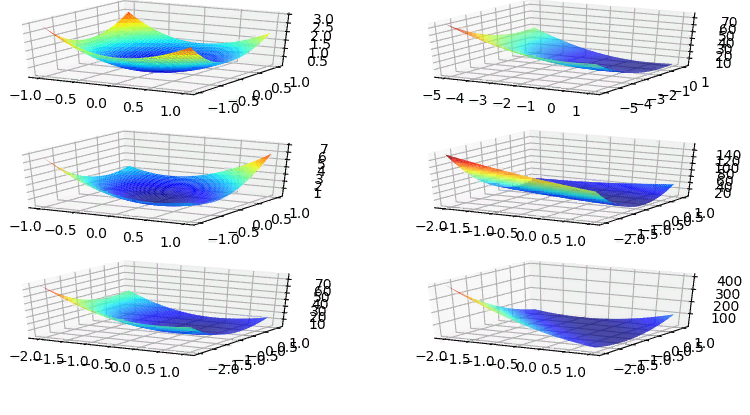
\includegraphics[scale=0.6]{tests/Examples.png}}
\caption{Examples of tests functions}
\label{fig:examples}
\end{figure}

We will use $a$ and $b$ from $[1, 2]$ and $N = 2$. Let's solve task of minimization function $f$ with different parameters on square $[0,1]^2$ through new method and compares number of iteration with estimate~\eqref{NI1}.

Result of the test you can see on fig.~\ref{fig:image}.

\begin{figure}[h!]
\center{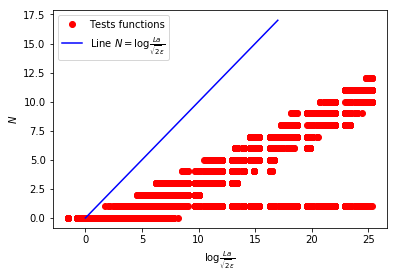
\includegraphics[scale=0.7]{tests/Test_results.png}}
\caption{Tests results for iterations number}
\label{fig:image}
\end{figure}

On graphic $N$ is number of done iterations for accuracy $\epsilon$, $\log_2\frac{La}{\sqrt{2}\epsilon}$ is the parameter of tests tasks. Line $N = \log_2\frac{La}{\sqrt{2}\epsilon}$ is our estimates \eqref{NI1}.

We can see that there are tests points under this line. It confirms our estimates \eqref{NI1}.

\subsection{Comparison}

Let's compare experimentally work's time of gradient descent and method of halving square. We will compare it on optimization task for functions from previous subsection and random quadric function with positive semidifenite matrix:
\begin{equation}\label{ex_1}
f(x,y) = -A_1\sin\frac{\pi x}{a} - B_1\sin\frac{\pi x}{b} + \left(-A_2\sin\frac{\pi x}{a} - B_2\sin\frac{\pi y}{b} + A_2 + B_2 + D_2\right)^2,
\end{equation}
where $A_i, B_i. D_i\geq 0$ for all $i = \overline{1, 2}$ and $a, b \in [1,2]$.

\begin{equation}\label{ex_2}
f(x,y) = (Ax + By)^2 + Cx^2 + Dx + Ey+ F, C\geq 0
\end{equation}
Halving square will stop when current value will be no further than $\epsilon$ from optimal value. Gradient descent will stop when distance between current and previous value will be not more than $\epsilon$.

We will use gradient descent with a step $h_k = \frac{h}{\sqrt{k}} = \frac{a}{4\sqrt{k}}$, where $a$ is size of the square. Also we add limit $N_{max} = 1000$ on the iterations number for method of halving square, solving on segment and gradient descent.

When we compare two method we distinguish the following situations (similar name of situations on graphics):

\begin{itemize}
\item Type 1 (T1) - tasks which gradient descent completed but halving square was not complete,
\item Type 2 (T2) - gradient descent is faster than halving square,
\item Type 3 (T3) - work's times are approximately equal or time is too short to measure,
\item Type 4 (T4) - gradient descent is slower than halving square,
\item Type 5 (T5) - gradient descent was not complete but halving square completed,
\item Type 6 (T6) - both methods were not completed successfully
\end{itemize}


\subsubsection{Sinuses}  

As already mentioned in previous subsection, functions \eqref{ex_1} meet conditions of lemma 2, therefore, we can take any point from segment on each iteration in method of halving square. Using all written above we have following results (see fig.~\ref{comp_sinuses}).

\begin{figure}[h!]
\center{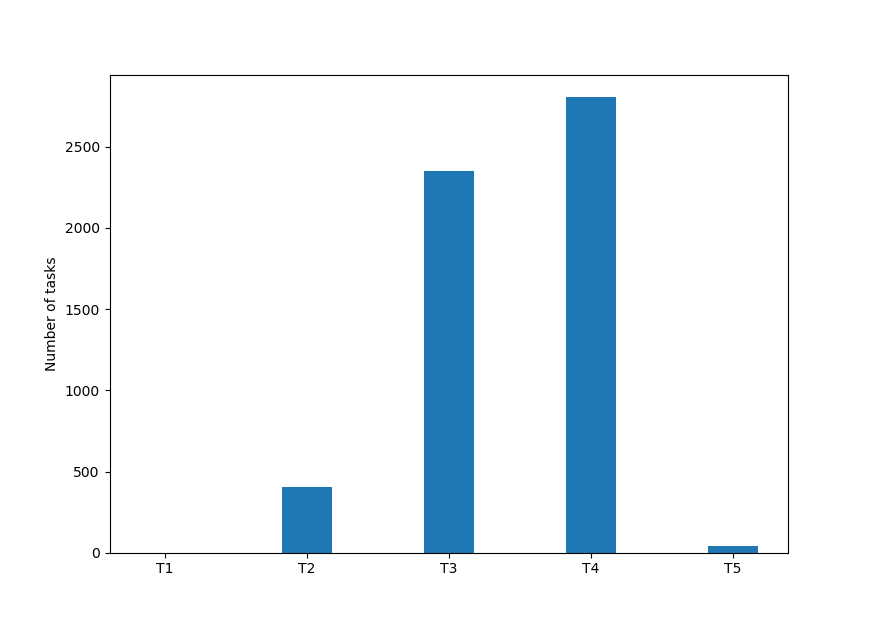
\includegraphics[scale=0.6]{tests/Comparison-sinuses.png}}
\caption{Tests results for comparison on sinuses}
\label{comp_sinuses}
\end{figure}

We can see that new method is not less efficient on the most tasks and more efficient on the task's half than gradient descent.

\subsubsection{Quadric functions}

Quadric functions do not always meet conditions of lemma 2, therefore, we can not think that error for task on segment can be very big. We can try to estimate this error but let's use for this task gradient descent with $|x-x_{prev}|<\delta$, where $\delta$ is much less than size of segment. In our experiments we will use $\delta = \frac{a}{400}$. Using it we have following results (see fig.~\ref{comp_pol}).

\begin{figure}[h!]
\center{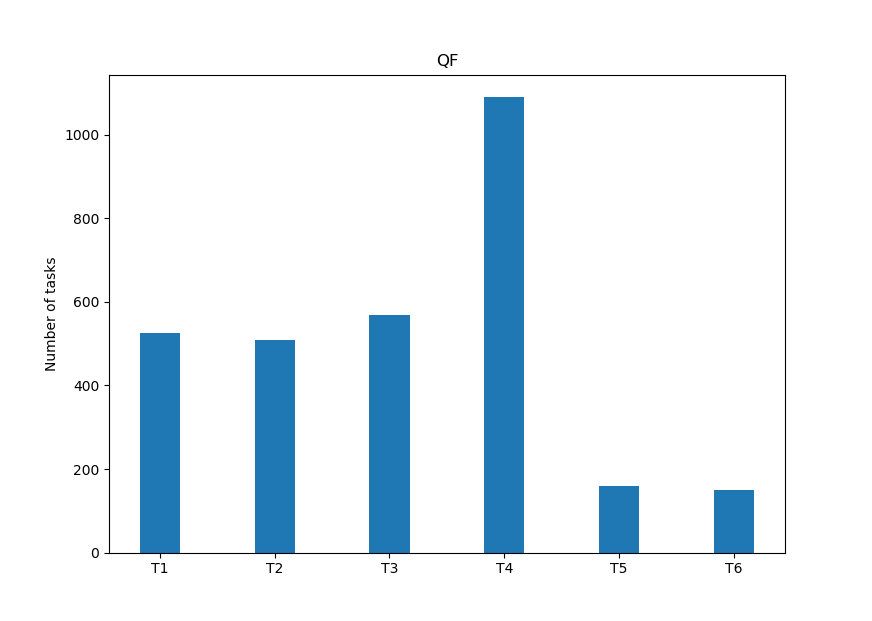
\includegraphics[scale=0.6]{tests/Comparison-pol.png}}
\caption{Tests results for comparison on quadric function}
\label{comp_pol}
\end{figure}

\end{document}
